\chapter{Datuen komunikazio asinkronoa: JSON, Ajax eta Promesak}

Nabigatzaileek kanpoko zerbitzariei web orriak eta gainontzeko elementuak eskatzeko HTTP protokoloa erabiltzen dute. Besterik ezean, nabigatzaileak eskaera sinkronoak egiten ditu: orria eskatu eta HTML kodearen zain geratzen da. Jaso ondoren, URLa aldatu eta beste orri bat eskatu ahalko dugu (aurrekoa gainidatziz).

\begin{figure}[ht]
	\centering
\begin{tikzpicture}
\node[anchor=south west,inner sep=0] (image) at (0,0)
   {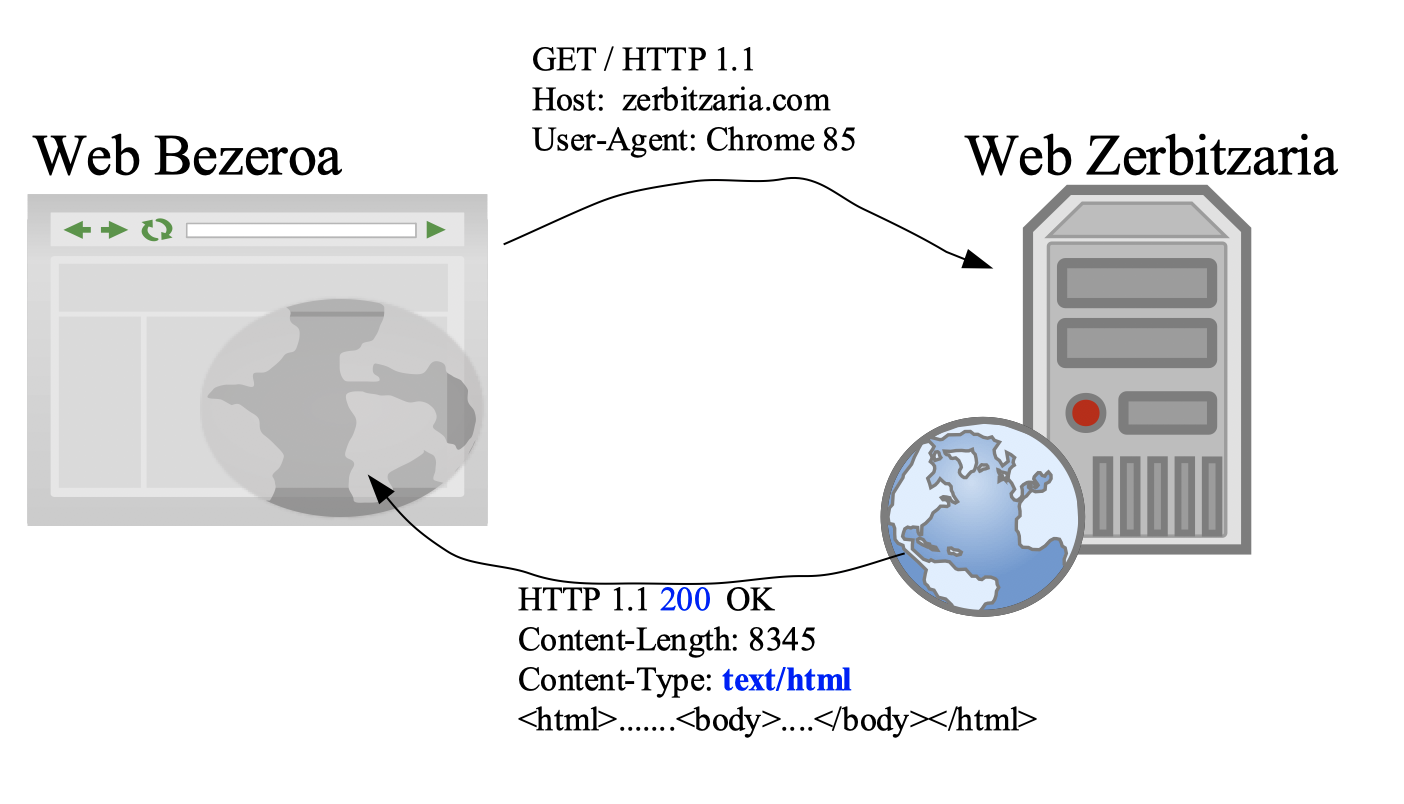
\includegraphics[trim=0cm 0cm 0cm 0cm, clip=true, width=0.75\textwidth]{img/http-protokoloa.png}};
\end{tikzpicture}
\caption{HTTP protokoloa eskaera sinkronoak eta asinkronoak egiteko erabil dezakegu.}
\label{fig:http-protocol}
\end{figure}

Baina batzuetan, behar dugun gauza bakarra ez dira web orri osoak izango, datu gordinak baizik. Are gehiago, batzuetan web orri baten barruan soilik datu zehatz bat bistaratu nahiko dugu, eta datua jasotzean ez dugu web orria zapaldu nahi, baizik eta datu hori pantailan ikusten dugun orriarekin integratu.

Adibidez, demagun Bilbo hiriaren GPS geokokapena non dagoen jakin nahi dugula. OpenWeatherMap izeneko zerbitzu bati, munduko hirien latitudea eta longitudea gordetzen dituen web zerbitzu bati, deitu diezaiokegu horretarako. Irudian ikusten dugun bezala, haren erantzuna ez da HTML formatuan etorriko, \index{JSON}JSON formatuan (JavaScript Object Notation) baizik. Horrez gain, eskaera ez dugu HTTP sinkrono bat erabiliz jaso nahi, baizik eta eskaera asinkrono batekin. Alegia, pantailan dugun orriaren edukia ordezkatu gabe, nabigatzaileak eskaera bat egingo dio OpenWeatherMap zerbitzuari eta JSON erantzuna jasotzean, Bilboko koordenatuak orrian bertan txertatu, dagokion lekuan.

HTTP eskaera asinkrono hauek \index{XHR}XHR (\index{XMLHttpRequest}XMLHttpRequest) edo AJAX \index{AJAX} izenarekin ezagutzen dira.

\begin{figure}[ht]
	\centering
\begin{tikzpicture}
\node[anchor=south west,inner sep=0] (image) at (0,0)
   {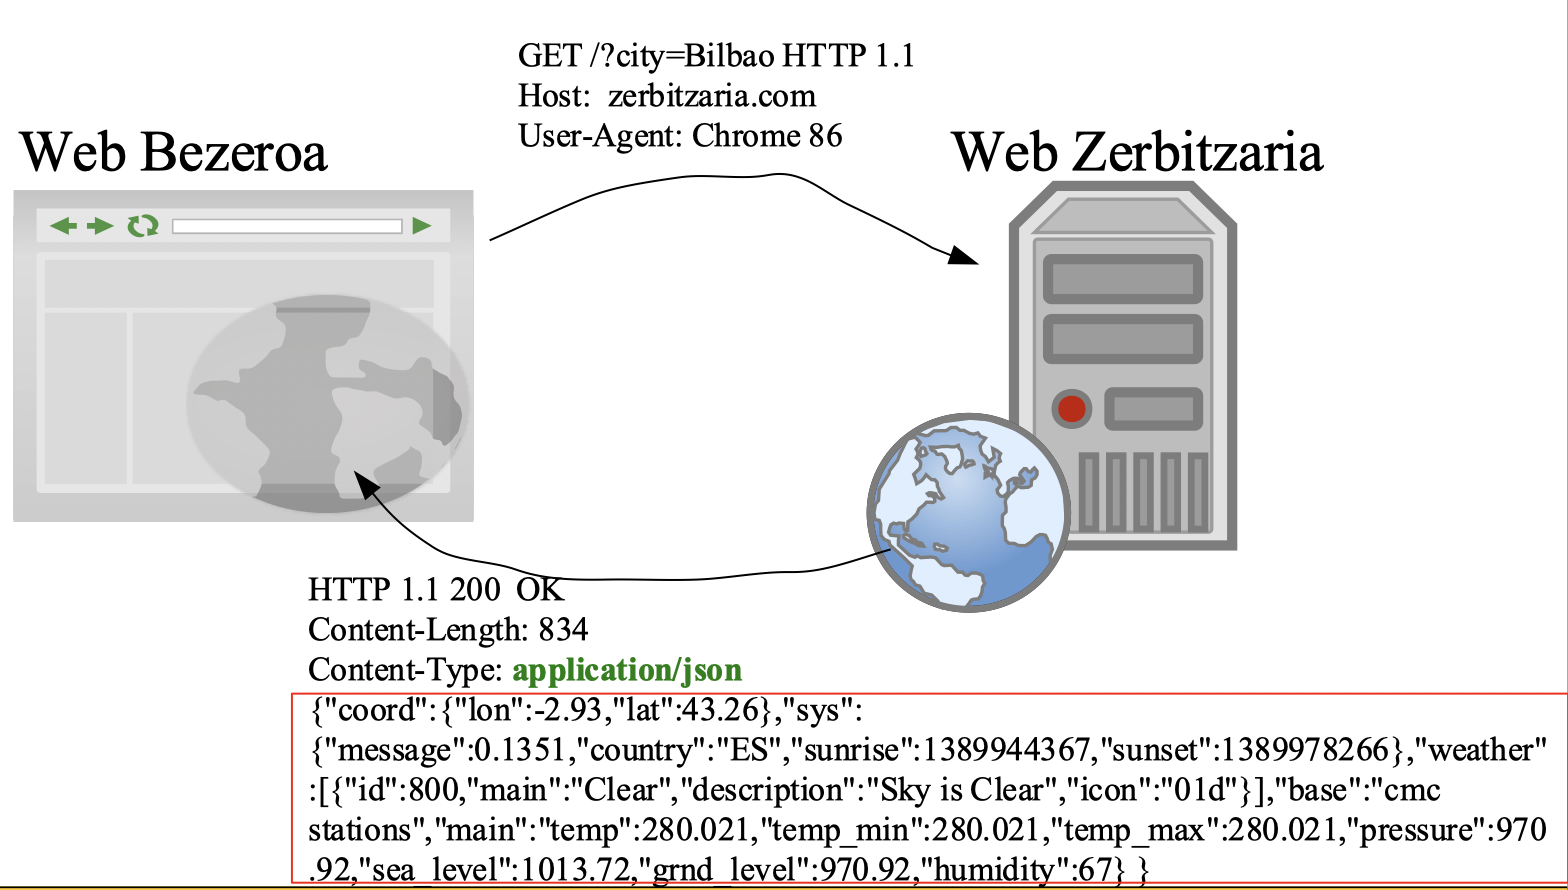
\includegraphics[trim=0cm 0cm 0cm 0cm, clip=true, width=0.75\textwidth]{img/xhr.png}};
\end{tikzpicture}
\caption{HTTP protokoloa erabiliz eskaera asinkronoak egiteari AJAX edo XHR deritzo. Adibidean, XHR dei bat egin diogu web zerbitzariari eta hark erantzuna bidali digu JSON formatuan.}
\label{fig:XHR}
\end{figure}

Adi! \index{XHR} XHR eskaerak egitean ez dugu zertan XML erabili. Hasieran XML Interneteko formatu estandarra bazen ere, gaur egun gehien erabiltzen den formatua JSON da eta, berez, XHR eskaeretan XML edo JSON jaso dezakegu.

Orain dela urte batzuk AJAX edo XHR eskaera bat egiteko kodea nahiko korapilatsua zen:

\begin{minipage}{\linewidth}
\begin{lstlisting}[language=JavaScript]
// zerbitzaria eta eskaera zehaztu
let url = "http://api.openweathermap.org/data/2.5/weather? q=Bilbao,es";

// Eskaera kudeatzeko XHR objektua sortu
let kontsulta = new XMLHttpRequest();

// URL horri eskaera egiteko GET metodoa erabiliko dugula zehaztu
kontsulta.open("GET", url);

//  eskaera asinkronoaren erantzuna kudeatuko duen funtzioa zehaztu
kontsulta.onload = function() {
  if (kontsulta.status == 200) {
    console.log("Arrakastaz egikaritutako kontsulta");
    console.log( kontsulta.responseText );
  }
};
// bukatzeko, eskaera jaurti besterik ez zaigu falta 
kontsulta.send();
\end{lstlisting}
\end{minipage}

AJAX eskaera baten erantzuna JSON formatuan baldin badator ere (ikus \ref{fig:XHR}. irudia), \textit{string} huts bat da. Modu eroso batean tratatu nahi badugu, JSON objektu bihurtu beharko dugu.
Adibidez, aurreko kode zatian, \index{responseText}\textit{kontsulta.responseText} katea JSON objektu bihurtzeko, \index{JSON.parse}\textit{JSON.parse} metodoa erabili beharko dugu.

\begin{verbatim}
    let erantzuna = JSON.parse(kontsulta.responseText);
\end{verbatim}

Gaur egun, kode hori guztia asko laburbil daiteke \index{fetch APIa}\textit{fetch} APIarekin. Izan ere, aurreko AJAX eskaera egiteko eta JSON formatura bihurtzeko, nahikoa litzateke lerro bakar hau exekutatzea (ikus \ref{fig:fetchAPI}. irudia):

\begin{verbatim}
fetch("http://api.openweathermap.org/data/2.5/weather?
q=Bilbao,es").then( r => r.json())
\end{verbatim}


\begin{figure}[ht]
	\centering
\begin{tikzpicture}
\node[anchor=south west,inner sep=0] (image) at (0,0)
   {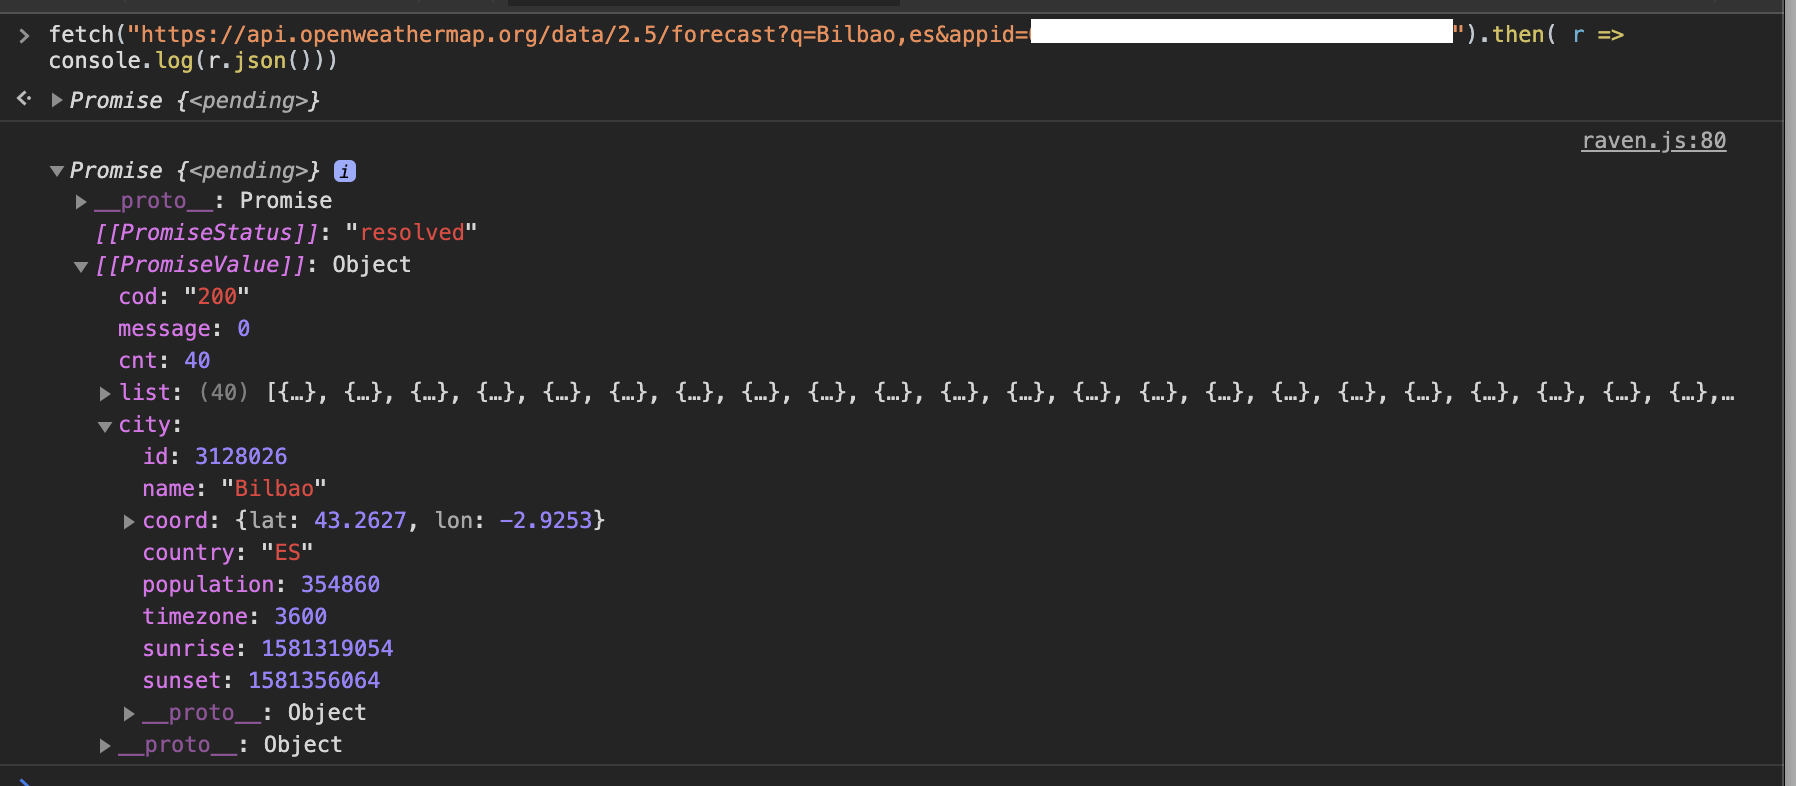
\includegraphics[trim=0cm 0cm 0cm 0cm, clip=true, width=0.75\textwidth]{img/openweatherfetch.png}};
\end{tikzpicture}
\caption{OpenWeatherMap (OWM) zerbitzuari AJAX eskaera bat egiteko HTML5ek eskaintzen duen \textit{fetch} APIa erabil dezakegu. Adi, doako API key bat eskatu beharko baitugu lehenengo OWM webgunean.}
\label{fig:fetchAPI}
\end{figure}

\index{Promise}\index{Promesak}
\section{Promesak}
Promes baten funtzionamendua ondo ulertzeko adibide bat ekarriko dugu. Irudi bat kargatu nahi dugu dinamikoki, promes baten bidez. Irudia deskargatu eta prest dagoenean dokumentuari erantsiko diogu DOM erabiliz, honela:

\begin{lstlisting}[language=JavaScript]
loadImage('https://developers.google.com/web/images/ web-fundamentals-icon192x192.png').
	then( image => document.body.appendChild(image) )
\end{lstlisting}

loadImage() irudia kargatzeko funtzioa da, promes bat itzultzen duena. Promesa betetzean (\textit{then} klausulan) document.body atzitu eta irudia erantsiko diogu .


\begin{lstlisting}[language=JavaScript]
function loadImage(url){
	return new Promise(resolve => {
		const image = new Image();
		image.addEventListener('load', () => {
			resolve(image);
		});
		image.src = url;
		});
}
\end{lstlisting}

loadImage() funtzioak, hortaz, URL bat hartzen du (irudiaren URLa) parametro gisa eta promes bat bueltatzen du. Promesak, aldiz, parametro gisa funtzio bat hartzen du ( \textit{.then} klausularen barruan definitu duguna aurreko kode zatian). Promes batek beti deituko dio parametro gisa jasotzen duen \textit{resolve} funtzioari, promesa betetzen denean.

Gure adibidean, noiz beteko da promesa? Lehenengo irudi bat sortzen dugu (new Image()). Jarraian, gertaera-kudeatzaile bat esleitzen diogu irudiari (image.addEventListener), irudia URLtik jaitsi eta prest dagoenean exekutatuko dena (onLoad). Kudeatzaile horrek deituko dio \textit{resolve} funtzioari. Noiz? image.src = url; komandoak irudia kargatzen bukatzen duenean (irudiaren iturria URLtik jaistean eta prest dagoenean). Ohart zaitez azken komando hori asinkronoa dela, alegia, badakigu noiz hasten den (komandoa exekutatzen hasten denean), baina ez noiz bukatzen den zehazki (denbora gutxiago edo gehiago har dezake irudia deskargatzeko konexio-kalitatearen arabera, adibidez).

Hurrengo irudian (\ref{fig:fetchAPI}. irudian), exekutatu dugun promesaren emaitza irudikatzen da. Zehazki, \hlc[lightgray]{fetch()} metodoaz dei asinkrono bat egin dugu eta promes bat jaso dugu. Promesa betetzean (\textit{fetch().then( r )} klausularen barruan gaudenean, non r jaso dugun erantzuna den)  erantzun bat aurkituko dugu. Erantzun hori JSON formatura bihurtu dugu (r.json() erabiliz). Orain, erantzuna JSON objektua denez, oso modu erosoan trata dezakegu. Adibidez, latitudearen eta longitudearen koordenatuak lortzeko, objektua.city.coord erabiliko genuke. Ikus hurrengo kode zatia:

\begin{lstlisting}[language=JavaScript]
fetch("https://api.openweathermap.org/data/2.5/forecast?
q=Bilbao,es&appid=XXXXXXXXXXXXXX").then( r => r.json()).then( objektua => {
  console.log(objektua);
  console.log(objektua.city.coord);
})
\end{lstlisting}

JavaScript-en edozein objektu JSON formatura bihur dezakegu eta hortik String arrunt batera \index{JSON.stringify}\hl{JSON.stringify} metodoa erabiliz (serializazioa deitzen zaio prozesu horri). Adibidez:

\begin{lstlisting}[language=JavaScript]
let liburu = new Liburu("Dublinés", "Alfonso Zapico", 18);
let jsonLiburua = JSON.stringify(liburu);
// orain jsonLinburua JSON formatuan dagoen String bat da
console.log(jsonLiburua);
// {"izenburua": "Dublinés", "egilea": "Alfonso Zapico",
// "salneurria": 18}
\end{lstlisting}

\section{Fetch APIa}

Fetch APIarekin eskaera asinkronoak egin ditzakegu, bai GET nola POST metodoak erabiliz (besteak beste). Ikus ditzagun adibide batzuk.

\subsection{Fetch APIa GET eskaerak egiteko}

OpenLibrary zerbitzuak eskaintzen duen APIa erabiliz liburu baten datuak jasoko ditugu fetch dei batekin:

\begin{lstlisting}[language=JavaScript]
fetch(
'https://openlibrary.org/api/books? bibkeys=ISBN:0451526538&format=json').
then( r => r.json() ).
then( datuak => { 
 console.log(datuak) 
 })
\end{lstlisting}

fetch egin ondoren, erantzun gordina jasoko dugu r parametroan. Parametro horren edukia JSON objektu bat denez, r.json() erabiliko dugu erantzuna JSON bihurtzeko. Jarraian, datuak izeneko parametroan jasoko dugu JSON objektua eta kontsolatik bistaratuko dugu, honako emaitza jasoz:

\begin{lstlisting}
{"ISBN:0451526538": 
{"bib_key": "ISBN:0451526538", 
"preview": "noview", 
"thumbnail_url": "https://covers.openlibrary.org/b/id/295577-S.jpg",
"preview_url": "https://openlibrary.org/books/OL1017798M/ The_adventures_of_Tom_Sawyer", 
"info_url": "https://openlibrary.org/books/OL1017798M/ The_adventures_of_Tom_Sawyer"
}}
\end{lstlisting}

Erantzun horretan thumbail\_url edo liburu-azalaren irudi txikia eskuragarri izango dugu. Beste \hl{fetch()} dei batekin jaso eta uneko orrian txertatuko dugu (\ref{fig:fetchAPIwebkontsola}. irudia):

\begin{lstlisting}[language=JavaScript]
fetch(
'https://openlibrary.org/api/books? bibkeys=ISBN:0451526538&format=json').
then( r => r.json() ).
then( datuak => { 
     let thumbnail_url = datuak["ISBN:0451526538"].thumbnail_url;
     let irudia = new Image(); irudia.src= thumbnail_url; document.body.appendChild( irudia );
 })
\end{lstlisting}

\begin{figure}[ht]
	\centering
\begin{tikzpicture}
\node[anchor=south west,inner sep=0] (image) at (0,0)
   {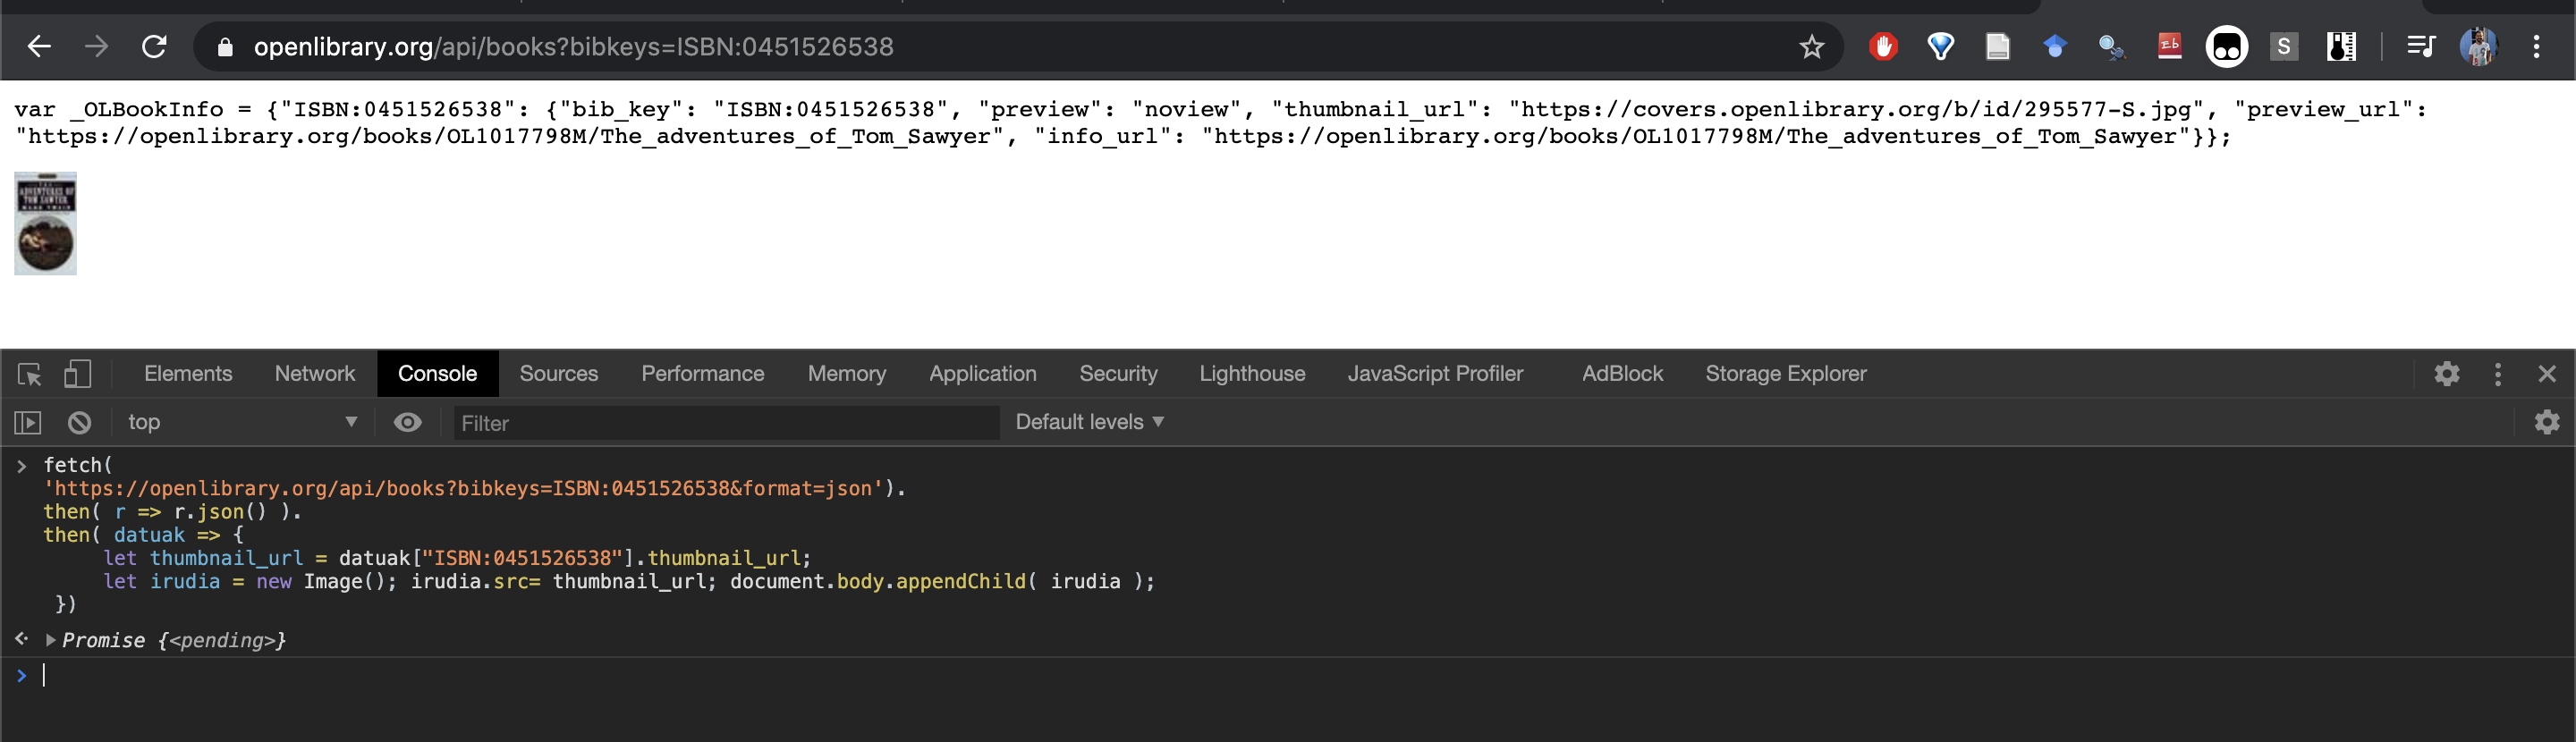
\includegraphics[trim=0cm 0cm 0cm 0cm, clip=true, width=1.0\textwidth]{img/fetch_webkontsola.png}};
\end{tikzpicture}
\caption{Fetch APIa erabiliz API bat kontsultatu eta erantzuna \textit{parseatu} ondoren, bertan zegoen irudi bat dokumentuan txertatu dugu. Probak egiteko nabigatzailearen web kontsola erabili dugu (ikus \ref{sec:webkontsola} atala).}
\label{fig:fetchAPIwebkontsola}
\end{figure}

\subsection{Fetch APIa POST eskaerak egiteko}

Fetch APIa POST eskaerak egiteko ere erabil daiteke. Horretarako, URLaren ondoren JSON objektu gisa parametroak pasa diezazkiokegu, \textit{method} eta \textit{body} atributuetan. 

Adibide gisa, httpbin.org/post helbidera (bidaltzen diogun guztia erantzun gisa errepikatuko du) POST eskaera bat bidaliko dugu, aldagai1=balio1 eta aldagai2=balio2 parametroekin:

\begin{minipage}{\linewidth}
\begin{lstlisting}[language=JavaScript]
fetch("https://httpbin.org/post", 
{ 
 method: 'POST',
 body: 'aldagai1=balio1&aldagai2=balio2'
}).then( resp => resp.text()).
then( erantzuna => console.log(erantzuna))
\end{lstlisting}
\end{minipage}

Eta erantzun gisa, honakoa jasoko dugu:

\begin{lstlisting}[language=JavaScript,numbers=none]
{
  "args": {}, 
  "data": "aldagai1=balio1&aldagai2=balio2", 
  "files": {}, 
  "form": {}, 
  "headers": {
    "Accept": "*/*", 
    "Accept-Encoding": "gzip, deflate, br", 
    "Accept-Language": "eu,en-US;q=0.9,en;q=0.8,es;q=0.7",
    "Cache-Control": "no-cache", 
    "Content-Length": "31", 
    "Content-Type": "text/plain;charset=UTF-8", 
    "Host": "httpbin.org", 
    "Origin": "chrome-search://local-ntp", 
    "Pragma": "no-cache", 
    "Sec-Fetch-Dest": "empty", 
    "Sec-Fetch-Mode": "cors", 
    "Sec-Fetch-Site": "cross-site", 
    "User-Agent": "Mozilla/5.0 (Macintosh; Intel Mac OS X 10_15_4) AppleWebKit/537.36 (KHTML, like Gecko) Chrome/83.0.4103.97 Safari/537.36", 
    "X-Amzn-Trace-Id": "Root=1-5edfaeca-dbf4fb5585f92c45ae2efda3"
  }, 
  "json": null, 
  "origin": "47.63.89.49", 
  "url": "https://httpbin.org/post"
}
\end{lstlisting}

\section{Ariketak}

Gai honetan zenbait teknologia eta teknika berri landu dira. JSON, AJAX, Fetch APIa eta Promesak. Horiek guztiak ondo ulertzeko ezinbestekoa da praktikatzea. 

\begin{enumerate}
    \item GDAX webguneak kriptotxanponen prezioa ezagutzeko API bat eskaintzen du. Adibidez, URL honi deituz \href{https://api.gdax.com/products/btc-eur/ticker}{https://api.gdax.com/products/btc-eur/ticker} \faBitcoin itcoin  baten prezioa (\faEuro urotan) emango digu, JSON formatuan (besteak beste, hainbat datu eskaintzen baititu dei horren erantzunak).
    
    \begin{figure}[ht]
	\centering
\begin{tikzpicture}
\node[anchor=south west,inner sep=0] (image) at (0,0)
   {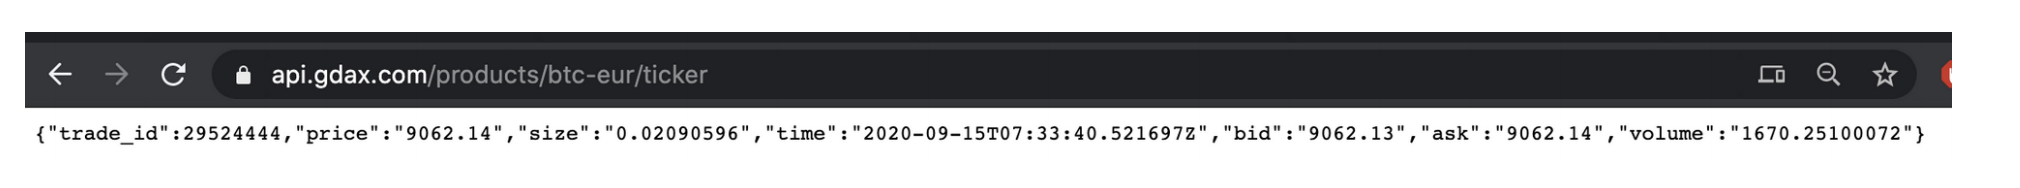
\includegraphics[trim=0cm 0cm 0cm 0cm, clip=true, width=1.0\textwidth]{img/json/json_ariketa_1.png}};
\end{tikzpicture}
\caption{JSON erantzun ezberdina jasoko dugu exekutatzen dugun guztietan, kriptotxanpon baten balioa une oro aldatzen baita.}
\label{fig:jsonariketa1}
\end{figure}

\faBitcoin itcoin baten prezioa dinamikoa da, egunean zehar hainbat aldiz aldatuko da (berez segundoero!).

fetch APIa erabiliz aurreko URLari deitu eta kontsolan idatzi \faBitcoin itcoin baten uneko prezioa.

\item loadImage() metodoa txantiloi gisa erabiliz (gogoratu gai honi dagokion kapituluan azaltzen dela bere funtzionamendua):

\begin{lstlisting}[language=JavaScript,numbers=none]
function loadImage(url){
   return new Promise(resolve => {
      const image = new Image();
      image.addEventListener('load', () => {
         resolve(image);
      });
      image.src = url;
});
}

loadImage('https://developers.google.com/web/images/ irudia.png').
then( image => document.body.appendChild(image) )
\end{lstlisting}

Inplementa ezazu loadAudio(url) izeneko beste funtzio bat, non parametro gisa audio-fitxategi baten URLa ematen zaion eta audio hori memorian kargatzen duen. Funtzioa inplementatu ondoren, dei honen bidez audioa entzun beharko litzateke:

\begin{lstlisting}[language=JavaScript,numbers=none]
loadAudio('https://zerbitzaria.com/audioa.mp3').then( audioa => audioa.play() );
\end{lstlisting}



\end{enumerate}